\documentclass[12pt, oneside, a4paper]{article}
\usepackage{afterpage}
\usepackage{amsmath}
\usepackage[a4paper]{geometry}
\usepackage{fullpage}
%\usepackage{listings}
%\usepackage{listingsutf8}
\usepackage{float}
\usepackage{hyperref}
\usepackage{minted}
\usepackage{fvextra}
\usepackage{multirow}
\usepackage[dvips]{graphicx}
\usepackage[utf8]{inputenc}
\usepackage[russian]{babel}
\usepackage{nccmath}
\usepackage{graphicx}
\usepackage[gray]{xcolor}
\graphicspath{{./}}
\begin{document}
\setminted[python]{breaklines=true}
\usemintedstyle{trac}
%\setmonofont[Scale=0.9,BoldFont={Inconsolata Bold}]{Inconsolata}
%ИСПОЛЬЗУЙ MINTED -shell-escape!!1!

\frenchspacing
\tableofcontents
\newpage
\section{Постановка задачи}
Для данного набора экспериментальных данных, характеризующих дыхание больного
человека, требуется построить странный аттрактор и найти его фрактальную
размерность. В наборе имеется 7341 значение.
\section{Теоретическая часть}
Одним из видов фрактальной размерности странного аттрактора является корреляционная размерность, которая характеризуется количеством
точек, попадающих в некоторую сферу или куб радиусом $\varepsilon$ вокруг каждой точки траектории движения поверхности, при стремлении радиуса к нулю.
Уравнение корреляционной размерности выглядит следующим образом:
\begin{eqnarray}
    d &=& \lim_{\varepsilon \rightarrow 0}
    \frac{\ln C(\varepsilon)}{\ln(\varepsilon)}\\
    C(\varepsilon) &=& \lim_{N \rightarrow \infty} \sum_{i = 1}^N 
    \sum_{\substack{j = 1 \\ i \neq j}}^N
    H(\varepsilon - \|x_i - x_j\|)
\end{eqnarray}

Для одновременного ряда для построения аттрактора и нахождения его размерности
используется псевдофазовое пространство, которое строится методом задержек:
\begin{equation}
    F(x_1, x_2, x_3,\dots) = F(x(\tau), x(\tau + T), x(\tau + 2T),\dots)
\end{equation}
Соответственно каждая точка аттрактора имеет 
следующие координаты в пространстве:
\begin{equation}
    \vec{x_i} = (x(\tau), x(\tau + T), x(\tau + 2T), \dots)
\end{equation}
Экспериментальные зависимости показывают, что для того, чтобы определить 
размерность аттрактора, для временного ряда, необходимо исследовать ассимптотику изменения фрактальной размерности аттрактора в зависимости от увеличения размерности псевдофазового пространства, в котором находится сам странный аттрактор.
\newpage
\section{Практическая часть}
\subsection{Выбор шага для метода задержек}
Используя метод задержек, в теории, нам необходимо лишь выполнение условия
не совпадения шага с частотой внешнего воздействия. Однако на практике, для
получения более адекватных результатов, также требуется и выбрать достаточно 
большой шаг. Адекватные результаты для данного аттрактора показывает выбор 
задержки, равный десяти периодам замерений. Это указывается явно в параметре 
\textit{\_\_tau} в программе.
\subsection{Нахождение оптимального размера $\varepsilon$}
Поскольку мы не знаем точности прибора, частоту измерений и прочих параметров, 
влияющих на фиксирование экспериментальных результатов, нам необходимо для 
начала подобрать параметр $\varepsilon$ для фрактальной размерности. Участок, в 
котором мы можем выбрать данный параметр может быть достаточно большим:
минимальная граница должна включать в себя как минимум еще одну точку, помимо
центра сферы или куба, максимальный размер может охватывать полноценную 
структуру. Тем не менее, в экспериментальных данных минимальный размер может 
быть ограничен шумами в измерениях.

Тем не менее, очевидно, что на некотором допустимом участке, 
при большом количестве измерений, размерность почти не будет отличаться и 
будет близка к фактической. Для того, чтобы определить этот участок, построим
зависимость параметра С от $\varepsilon$ в логарифмических координатах, и
выберем точку на этом участке, которая будет использована в дальнейших 
рассчетах.

Для всех вычислений была написана программа, в ней эту операцию выполняет 
функция \textit{build\_variation\_of\_eps}. 
Функция вычисляет зависимость и строит
график в логарифмических координатах. Результат работы программы на участке от 
0.00018 до 2.61 выглядит следующим образом: 
\begin{figure}[!h]
    \caption {Зависимость параметра $\ln(C)$ от параметра $\ln{\varepsilon}$ }
    \centerline{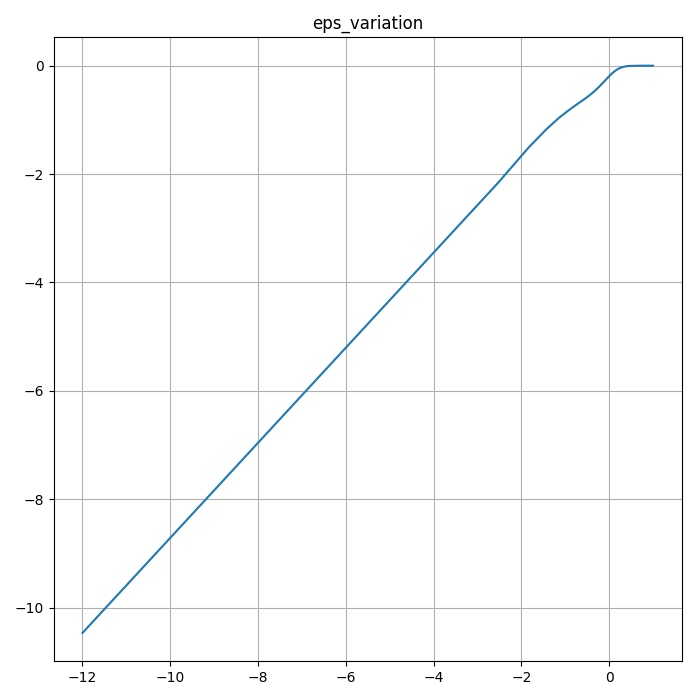
\includegraphics[scale = 0.72]{../results/lce.png}}
\end{figure}
\newpage
Для дальнейших расчетов, параметр $\varepsilon$ был выбран равным $e^{-4}$.
\subsection{Нахождение аппроксимированной размерности аттрактора}
Как было указано в теоретической части, нахождение фрактальной
размерности аттрактора, когда нам неизвестно количество фактических уравнений
и параметров нелинейной хаотической системы, требует исследования ассимптотики
данного процесса. Это достигается с помощью нахождения фрактальной размерности
в псевдофазовых пространствах с разными размерностями.

Функция \textit{build\_variation\_of\_dim}, для построения графика зависимости приведена в программе.
Её работа тривиальна, она рассчитывает 
размерность аттрактора для каждого измерения, от минимального до максимального,
после чего строит график. Нам же требуется выбрать само значение аттрактора.

График зависимости приведен ниже:
\begin{figure}[!h]
    \caption {Зависимость корреляционной размерности от размерности псевдофазового пространства}
    \centerline{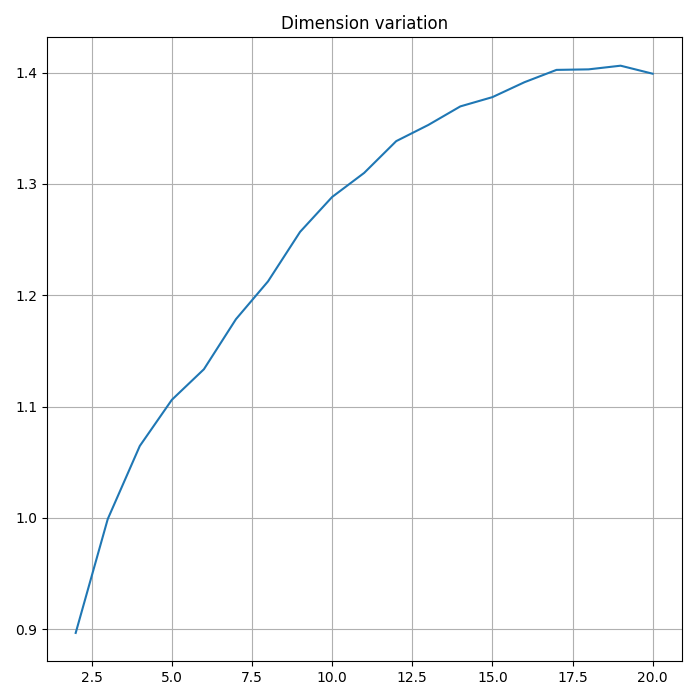
\includegraphics[scale = 0.8666]{../results/dim.png}}
\end{figure}

Как видно из графика, значение фрактальной размерности стремится к значению 1.4. Действительно, на 19 итерации значение размерности равно 1.406. Возьмем это значение за значение фрактальной размерности аттрактора.

\subsection{Построение странного аттрактора}
Поскольку получившееся значение фрактальной размерности аттрактора у нас 
меньше двух, но больше единицы, строить аттрактор имеет смысл в 
двухмерной псевдофазовой плоскости. Аттрактор строится также методом 
задержек, который был изложен в теоретической части.gt

Для построения аттрактора была написана функция \textit{stage3}, 
результат работы которой представлен ниже:
\begin{figure}[H]
    \caption {Странный аттрактор}
    \centerline{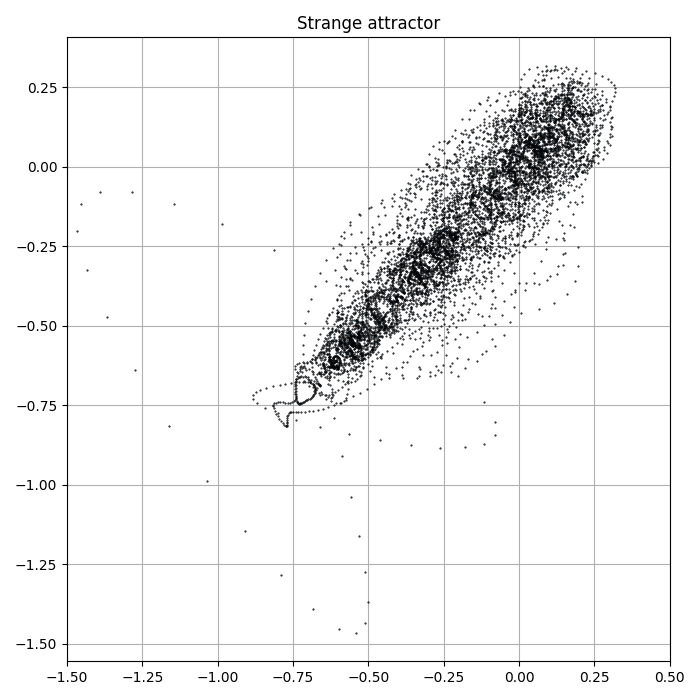
\includegraphics[scale = 1.0]{../results/sat1.png}}
\end{figure}
Как можно видеть, у аттрактора есть некоторая дуга, которая явно выбивается 
из общей тучности точек, притом в тучности заметны подобные эллиптические
фрактальные фигуры. Если рассмотреть график только в этой тучности, то там также
прослеживается фрактальная структура, похожая чем-то на сложную цепь.
Если начертить сами линии и просмотреть структуру непосредственно в приближении,
то можно увидеть повторяющие многократно друг друга со сдвигом эллипсы:
\afterpage{%
    \thispagestyle{empty}
    \begin{figure}[H]
    \caption {Участок странного аттрактора в тучности}
    \centerline{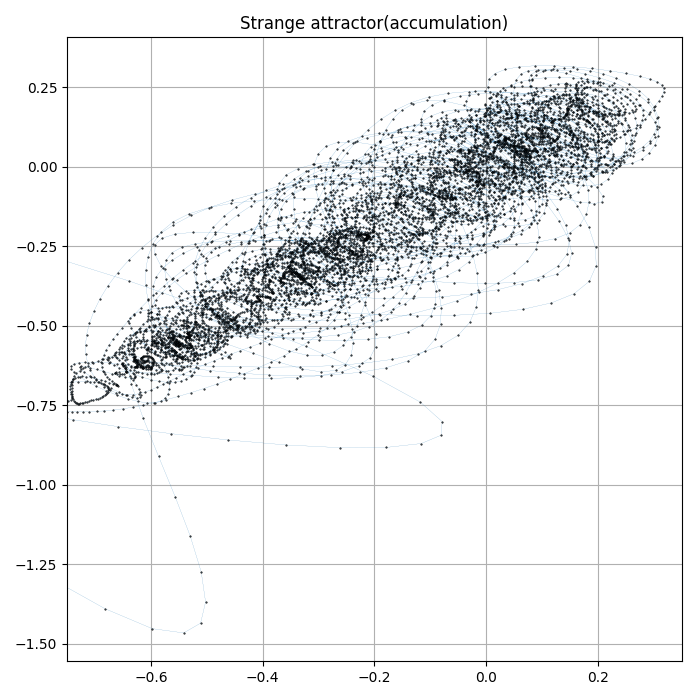
\includegraphics[scale = 0.66]{../results/sat2.png}}
    \caption {Приближение тучности:}
    \centerline{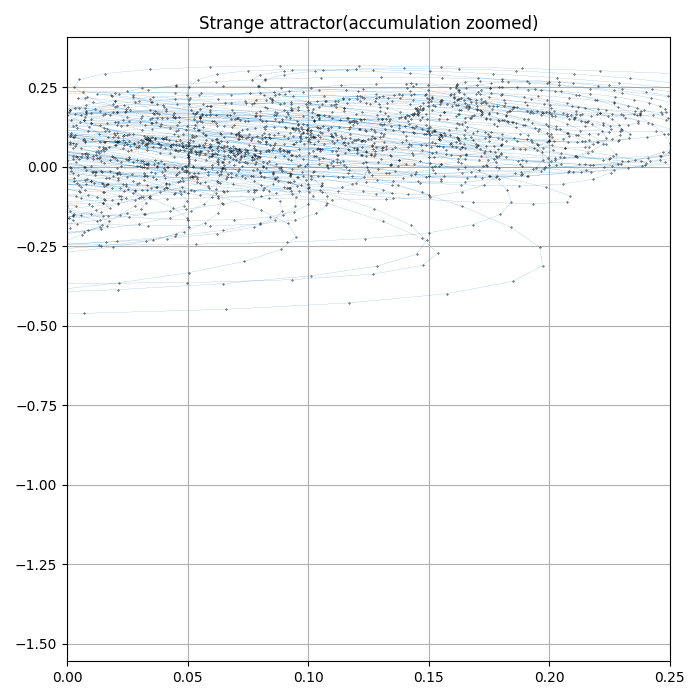
\includegraphics[scale = 0.66]{../results/sat3.png}}
\end{figure}
}
\pagebreak
\section{Вывод}
Проведя данные вычисления, мы можем явно убедиться в том, что процесс дыхания человека является хаотическим, а также в том, что структура странного аттрактора является фрактальной. Была также вычислена размерность аттрактора в псевдофазовом пространстве и построены зависимости параметра C от $\varepsilon$ и размерности аттрактора от размерности псевдофазового пространства.
\newpage
\section*{Приложение: код программы для решения задачи}
Для работы программы требуется установить интерпретатор языка Python, а также
с помощью пакетного менеджера pip поставить пакеты numpy и matplotlib. 
Альтернативно, можно поставить набор Anaconda, в который входит все вышеперечисленное.
\begin{minted}[breaklines]{python}
import numpy as np
import sys
import matplotlib
matplotlib.use('Agg')
import matplotlib.pyplot as plt

class file_printer:
    class __OnlyOne:
        def __init__(self):
            pass
    instance = None
    def __init__(self):
        if not file_printer.instance:
            file_printer.instance = file_printer.__OnlyOne()
    def __getattr__(self, name):
        return getattr(self.instance, name)
    def write_line(self, log_line):
        with open("log.txt", 'a') as f:
            f.write(log_line + '\n')

def delay_translate (src_vec, new_dim):
    '''
    Creates from [1xN] vec [Mx(N-M*__tau)] vec
    '''
    print("delay translate, tau = {}".format(__tau))
    result = list()
    for i in range (new_dim):
        tmp_vec = src_vec[i*__tau: len (src_vec) - (new_dim-i-1)*__tau]
        result.append (tmp_vec)
    return result

def distance_between_points (p1, p2):
    '''
    Calculates non-euclid distance between points
    (required by fractal_dimension calculator)'''
    #print("{} - {}".format(p1, p2))
    return abs (sum ([i - j for i in p1 for j in p2\
                    if p1.index (i) == p2.index (j)]))

def build_2d_plot (dataX, dataY, fig_name, ls = 'solid', marker = '.',
        left_xlim = None, right_xlim = None, lw = 1, ms = 0.5):
    '''builds a plot of dataX - dataY and save it to fig_name'''
    print("plotter")

    fig, m_graph = plt.subplots (1)
    m_graph.set_xlim(left_xlim, right_xlim)
    m_graph.plot (dataX, dataY, ls = ls, marker = marker, ms = ms, mec = 'black', lw = lw)
    #m_graph.set_ylim(ymin=0)
    m_graph.grid (True)
    m_graph.set_title (fig_name)

    fig.set_size_inches( 7, 7)
    fig.tight_layout ()
    fig.savefig (fig_name + ".png")


def heaviside_function (x):
    return int(x>=0)

def cr_function (src_vec, eps):
    transposed_vec = np.array (src_vec).T
    c_r = sum ( [heaviside_function(\
                    eps - distance_between_points (list(i), list(j)))\
        for i in transposed_vec for j in transposed_vec\
        if not np.array_equal (i, j)] )/((len(transposed_vec))**2)

    return c_r

def correlation_dimension (src_vec, eps):
    return np.log (cr_function (src_vec, eps))/np.log (eps)

def build_variation_of_eps (src_vec, dimension, eps_min, eps_max, iterations):
    dataY = list()
    dataX = list()
    formated_vec = delay_translate (src_vec, dimension)
    print("build_variation_of_eps")
    for eps in np.arange(eps_min, eps_max,(eps_max - eps_min)/iterations):
        c_temp = cr_function(formated_vec, eps)
        dataY.append (np.log (c_temp))
        dataX.append (np.log (eps))
        a = file_printer()
        a.write_line("x - {} || y - {}".format(eps, c_temp))
    build_2d_plot (dataX, dataY, "eps_variation")

def load_data (file_name):
    src_vec = list()
    with open (file_name) as f_in:
        while True:
            line = f_in.readline()
            if line == '':
                break
            src_vec.append (float(line))
    return src_vec

def stage_1():
    file_name = input ("data file name: ")
    src_vec = load_data (file_name)
    
    eps_min = float (input ("left boundary to search eps: "))
    eps_max = float (input ("right(exclusive) boundary to search eps: "))
    iterations = int (input ("iterations to search: "))
    build_variation_of_eps (src_vec, 2, eps_min, eps_max, iterations)

def build_variation_of_dim(src_vec, eps, min_dim, max_dim):
    dataX = list()
    dataY = list()
    for dim in range (min_dim, max_dim + 1):
        formated_vec = delay_translate (src_vec, dim)
        cr_temp = correlation_dimension (formated_vec, eps)
        dataX.append (dim)
        dataY.append (cr_temp)
        a = file_printer ()
        a.write_line ("{} - {}".format(dim, cr_temp))
    build_2d_plot (dataX, dataY, "Dimension variation")

def stage_2():
    file_name = input ("data file name: ")
    src_vec = load_data (file_name)
    eps = float (input ("eps of sphere(from stage 1): "))
    min_dim = int (input ("least dimension: "))
    max_dim = int (input ("biggest dimension: "))
    
    build_variation_of_dim(src_vec, eps, min_dim, max_dim)

    print("nope")
def stage_3():
    file_name = input ("data file name: ")
    src_vec = load_data(file_name)
    d2 = delay_translate(src_vec, 2)
    
    build_2d_plot(d2[0], d2[1], "Strange attractor", ls = 'None',
            left_xlim = -1.5, right_xlim = 0.5, ms = 1)
    build_2d_plot(d2[0], d2[1], "Strange attractor(accumulation)",  
            left_xlim = -0.9, right_xlim = -0.1, ms = 1, lw = 0.1)
    build_2d_plot(d2[0], d2[1], "Strange attractor(accumulation zoomed)", lw = 0.1,
            left_xlim = -0.5, right_xlim = -0.4, ms = 0.7)

if __name__=="__main__":
    stage = int (input ("select stage: "))
    if stage == 1:
        stage_1()
    elif stage == 2:
        stage_2()
    elif stage == 3:
        stage_3()
\end{minted}
\end{document}
